\section{$S$ is the solution set of a homogeneous quadratic}\label{sec:partb}
In this section we consider the case when
\[
	S = \{(x_1,\ldots,x_n) \mid Q(x_1,\ldots,x_n) = 0\}
\]
where $Q$ is a homogeneous quadratic. In order to compute $\Phi(\IND_S)$, we must determine $|\ker \lambda \cap S|$ for given $\lambda \in V^*$. If we think of elements of $V$ as column vectors, then elements $\lambda \in V^*$ can be thought of as row vectors, with
\[
	\ker \lambda = \langle \lambda \rangle^\bot = \{x \in V \mid \lambda x =0\}.
\]

We begin with an illustrative example over the reals before considering the situation over $\F_p$. Let $Q = 3x_1^2 + 3x_2^2 - 2x_3^2$. The conic $S = \{Q = 0\}$ is depicted in Figure~\ref{fig:conic-with-plane}.
\begin{figure}[h]
	\centering
	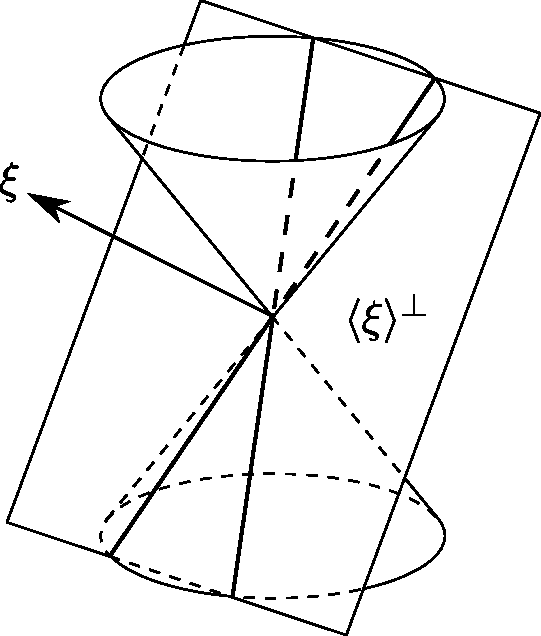
\includegraphics[width=0.6\linewidth]{conic-with-plane}
	\caption{}
	\label{fig:conic-with-plane}
\end{figure}
The intersection $\langle \lambda \rangle^\bot \cap S$ has three possible shapes:
\begin{itemize}
	\item a pair of lines intersecting at the origin (which is the case depicted with $\lambda = (0,-2,1)$),
	\item the origin alone (e.g. $\lambda = (0,0,1)$), and
	\item a single line, which happens when $\langle \lambda \rangle^\bot$ is tangent to the conic (e.g. $\lambda = (0,-\sqrt{3},\sqrt{2})$).
\end{itemize}
In fact, the set of $\lambda$ such that $\langle \lambda \rangle^\bot$ is tangent to the conic is given by
\[
	\left\{ \lambda = (\lambda_1,\lambda_2,\lambda_3) \mid \frac{1}{3} \lambda_1^2 + \frac{1}{3} \lambda_2^2 - \frac{1}{2} \lambda_3^2 = 0 \right\} \subset V^*.
\]
This is a conic in $V^*$, and it is dual to our original conic in a sense that we will soon explain. Let us we write $Q^*$ for the equation of this dual conic. Observe that $Q^*(0,-2,1) > 0$ while $Q^*(0,0,1) < 0$. It turns out that the sign of $Q^*(\lambda)$ is all one needs to classify the intersection $\langle \lambda \rangle^\bot \cap S$.

Now we consider the general situation in $n$ variables over $\F_p$. For convenience, we will assume that $p>2$. To a homogeneous quadratic
\[
	Q = \sum_{1 \leq i \leq j \leq n} c_{i,j} x_i x_j 
\]
we associate the $n\times n$ matrix $A$ whose entries are given by
\[
	a_{i,j} = \begin{cases}
		{c_{i,j}}/{2} & \text{if } i < j,\\
		c_{i,j} & \text{if } i = j, \text{ and}\\
		{c_{j,i}}/{2} & \text{if } i > j.
	\end{cases}
\]
Then, if $x = (x_1,\ldots,x_n)^\top$, we have
\[
	Q(x) = x^\top A x.
\]
The conic $S = \{Q = 0\}$ is \emph{non-degenerate} if the matrix $A$ is invertible. We will assume that this is the case.

\begin{defn}
	The \emph{orthogonal group of $A$}, denoted $O(A)$, is defined to be
	\[
		O(A) \coloneqq \{ g \in GL(V) \mid g^\top A g = A\}.
	\]
	Also define
	\[
		kO(A) \coloneqq \{ cg \mid c\in \F_p, g\in O(A)\}.
	\]
\end{defn}

We are interested in this group because elements of $kO(A)$ map $S$ to itself.
\begin{defn}
	A group $G$ acts \emph{transitively} on a set $S$ if for all $a,b\in S$, there exists $g\in G$ such that $g\cdot a = b$. Equivalently, the only orbit of the action is the entirety of $S$.
\end{defn}

\begin{prop}
	The group $kO(A)$ acts transitively on each of the following sets:
	\begin{enumerate}
		\item $S = \{x \in V \mid x\neq 0, x^\top A x = 0\}$,
		\item $\{ x\in V \mid x^\top A x \text{ is a nonzero square in } \F_p\}$, and
		\item $\{ x\in V \mid x^\top A x \text{ is not a square in }\F_p\}$.
	\end{enumerate}
\end{prop}
\begin{proof}
	It is an elementary fact that if $a,b\in \F_p$ are not squares, then $b/a \in \F_p$ is a square. Hence if $u,v\in V$ belong to the same set above, we can assume $u^\top A u = v^\top A v$ (as it can be achieved by scaling).
	
	If $u$ and $v$ are linearly dependent then the result is immediate, so suppose otherwise. Take a basis $\{u,v,e_3,\ldots,e_n\}$ and apply Gram-Schmidt to it, obtaining an orthogonal basis $\{u, w_2, w_3, \ldots,w_n\}$. Now consider the basis
	\[
		\{u,v,w_3,\ldots,w_n\}
	\]
	which has the property that
	\[
		w_i^\top A u = w_i^\top A v = w_i^\top A w_j = 0 \text{ for all } i \neq j, \text{ and }\\
		u^\top A u = v^\top A v.
	\]
	It is straightforward to verify that the linear transformation which interchanges $u$ and $v$ while fixing $w_3,\ldots,w_n$ is an element of $O(A)$.
\end{proof}